\subsection{Convenzioni e diagramma generale}
Ogni caso d'uso è descritto con: nome, attore, requisiti correlati, precondizioni, postcondizioni, flusso principale e flussi alternativi. I flussi alternativi sono numerati rispetto al passo in cui si innestano (es. \textbf{4a} è un'alternativa al passo 4; \textbf{4a.1}, \textbf{4a.2} sono i suoi passi).

\textbf{Precondizione comune.} In tutti i casi d'uso l'applicazione è avviata e l'archivio è stato caricato (ED4.2).

\textbf{Flussi alternativi comuni.} Per non ripeterli in ogni caso d'uso:

\begin{itemize}
\item \textbf{FC1 – Annullamento.} In qualsiasi passo in cui il sistema attende dati o una conferma, l'Operatore può annullare: il sistema chiude la finestra senza modificare l'archivio e il caso d'uso termina.
\item \textbf{FC2 – Errore di salvataggio.} Se il salvataggio dell'archivio su file non riesce, il sistema non applica l'operazione, mostra un messaggio di errore e il caso d'uso termina con l'archivio invariato (ED4.4).
\end{itemize}
Relazioni tra casi d'uso usate nei diagrammi:

\begin{itemize}
\item \textbf{\guillemotleft{}include\guillemotright{}} (freccia tratteggiata verso il caso d'uso incluso): il caso d'uso incluso è \textbf{sempre} eseguito come passo del caso d'uso base. VerificaSovrapposizioni è incluso dai due casi d'uso di inserimento, perché il controllo dei conflitti va fatto sempre.
\item \textbf{\guillemotleft{}extend\guillemotright{}} (freccia tratteggiata verso il caso d'uso esteso): il caso d'uso che estende viene eseguito \textbf{solo in certe condizioni}. CancellaPrenotazioniInCascata estende sia CancellaAula sia CancellaDocente (il comportamento è lo stesso); GestisciConflittiSerie estende InserisciPrenotazioneRicorrente; CancellaOccorrenzeSuccessive estende CancellaPrenotazione.
\end{itemize}
I diagrammi sono generati con PlantUML; i sorgenti (\texttt{.puml}) si trovano nel repository, nella cartella \texttt{docs/requisiti/diagrammi/}.

\begin{figure}[H]
\centering
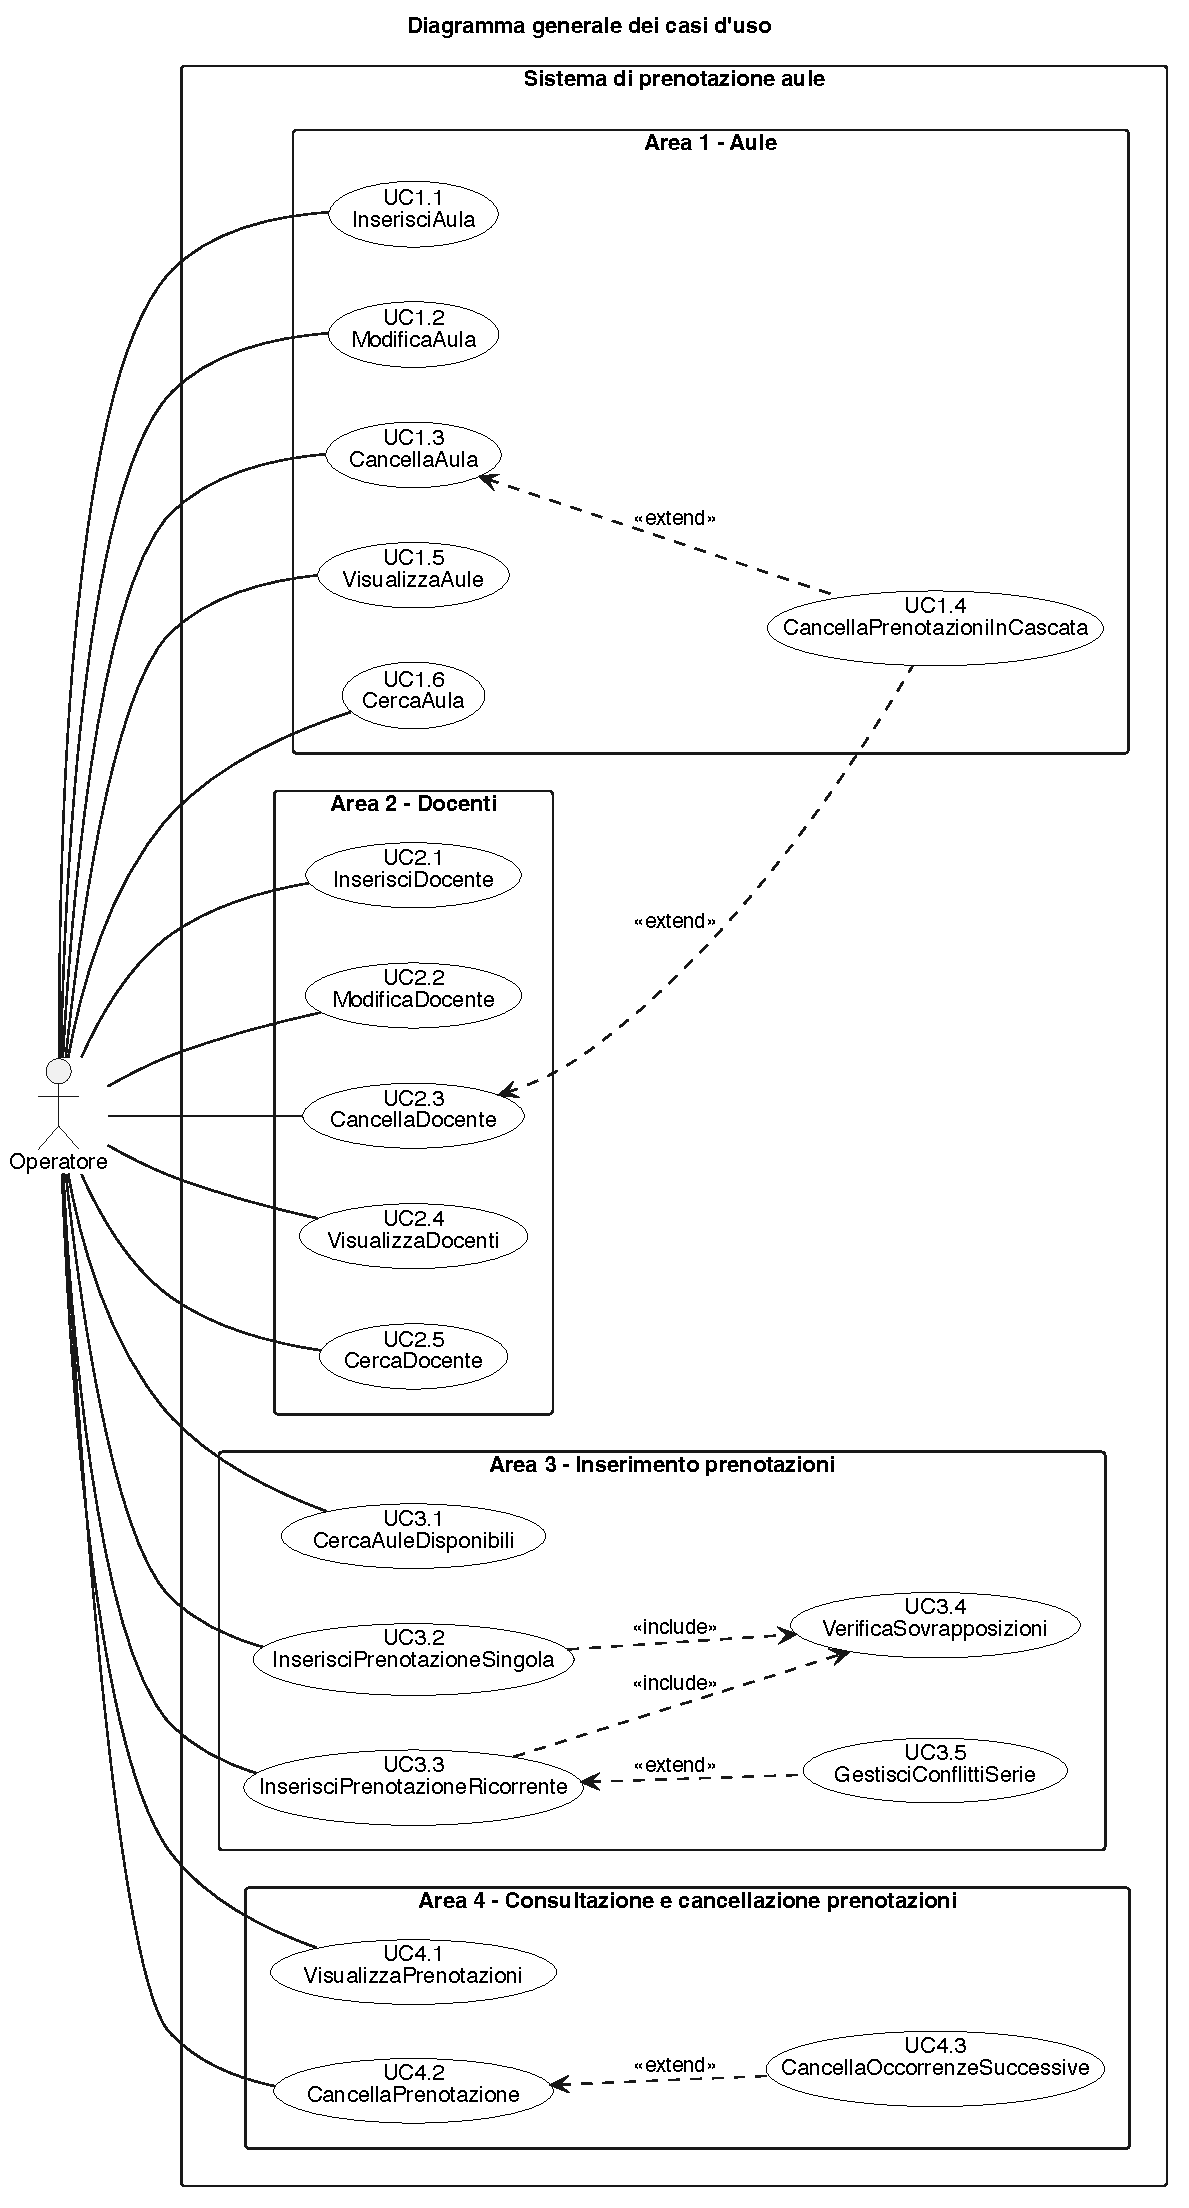
\includegraphics[width=\textwidth,height=0.8\textheight,keepaspectratio]{diagrammi/uc-generale}
\caption{Diagramma generale dei casi d'uso}
\end{figure}
